\chapter{Datenquelle 1: EU Verordnungen und Cellar}
\section{Europäische Verordnungen}

    Die regulative Grundlage für alle, in dieser Arbeit thematisierten, Anforderungen werden direkt oder delegiert in europäischen Verordnungen -- und jene konsolidierende Medien -- festgehalten.
    Die Arbeitsweise der EU und dessen beteiligte legislative Organe wird durch den \acf{EUV} und dem \acf{AEUV} festgelegt.
        
\subsection{Beteiligte Organisationen}
\subsubsection{Europäische Kommission}

    \begin{center}
        {\footnotesize(Art. 17 \ac{EUV})}
    \end{center}
    
    \noindent
    Die Europäische Kommission, mit Sitz in Brüssel, vertritt durch je ein Mitglied alle EU-Staaten (zzt.: 27). 
    Sie verfügt als einziges Organ über das Initiativrecht im Gesetzgebungsverfahren und kann – u.U. nach der Aufforderung von Rat, Parlament oder Bürgerinitiativen – einen Gesetzesvorschlag annehmen und diesen, in enger Zusammenarbeit mit den anderen Organen, durch den gesamten Gesetzgebungsprozess begleiten.
    \cite[Art. 17]{EUV}
    Weiter erlässt oder delegiert die Kommission zusammen mit den unter \ac{SES} definierten Ausschüssen und Agenturen Durchführungsvorschriften, welche zur Verwirklichung der in dem Rahmen definierten Interoperabilität dienen. (siehe \ref{ch:ir})
    
\subsubsection{Rat der Europäischen Union}

    \begin{center}
        {\footnotesize(Art. 16 \ac{EUV}, Art 137ff. \ac{AEUV})}
    \end{center}
    
    \noindent
    Der Rat der Europäischen Union – nicht zu verwechseln mit dem Europäischen Rat – ist ein legislatives Organ der EU mit Sitz in Brüssel, welches -- bis auf Ausnahmen -- zusammen mit dem Europäischem Parlament Rechtsakte beschließt.
    Der Rat der EU (auch Ministerrat) setzt sich aus je einem Vertreter auf Ministerebene der Mitgliedsstaaten zusammen. 
    Der Rat tritt hierbei in verschiedenen Fachformationen zusammen -- darunter auch Verkehr -- um die Interessen der Mitgliedstaaten in Bezug auf entwickelte Gesetzesakte zu erörtern.
    Im Weiteren arrangiert der Rat auch internationale Abkommen und Verträge mit Drittstaaten oder internationalen Organisationen.
    
\subsubsection{Europäisches Parlament}
    
    \begin{center}
        {\footnotesize(Art. 13, 14 Abs. 1 \ac{EUV}, Art 223f \ac{AEUV})}
    \end{center}
    
    \noindent
    Das Europäische Parlament setzt sich aus Vertretern der Unionsbürger:innen zusammen.
    Mitglieder des Parlaments werden in allgemeiner Wahl für eine Amtszeit von fünf Jahren gewählt.
    Die besondere Bedeutung im Rahmen europäischer Anforderungen kommt dem Parlament zu, da entsprechende Rahmenbedingungen\footnote{beispielsweise \ac{SES} Paket I \& II} der Verkehrspolitik in Kombination mit der Kommission, und in dem Rahmen des Ordentlichen Gesetzgebungsverfahrens (siehe \ref{ch:ord_ggv}), entwickelt werden.

\subsection{Ordentliches Gesetzgebungsverfahren} \label{ch:ord_ggv}
    
    Das \textit{ordentliche Gesetzgebungsverfahren} definiert seit dem Vertrag von Lissabon eine überarbeitete Version des Mitentscheidungsverfahrens \cite[Art. 294]{AEUV}, welches den Gesetzgebungsprozess gewisser Themenbereiche\footnote{darunter auch Verkehrspolitik} bestimmt. 
    
    Die wichtigsten Schritte des Verfahrens lassen sich wie folgt beschreiben:
    \begin{enumerate}
        \item Die Europäische Kommission unterbreitet dem Europäischen Parlament und dem Rat einen Vorschlag.
        \item Der Rat und das Parlament nehmen einen Gesetzgebungsvorschlag entweder in erster oder in zweiter Lesung an.
        \item Erzielen beide Organe in zweiter Lesung keine Einigung, wird ein Vermittlungsausschuss einberufen.
        \item Ist die vom Vermittlungsausschuss vereinbarte Fassung in dritter Lesung für beide Organe annehmbar, wird der Rechtsakt erlassen.
    \end{enumerate}

    \begin{figure}[H]
        \centering
        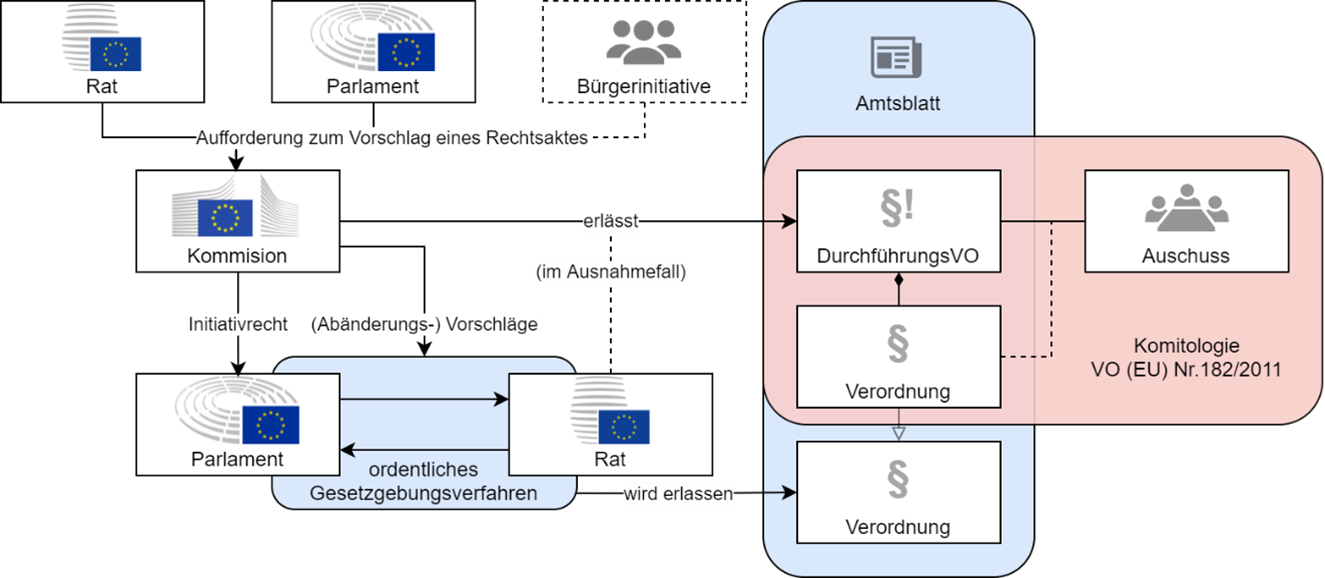
\includegraphics[width=\linewidth]{gfx/Gesegebungsprozess.png}
        \caption{Gesetzgebungsprozess der EU} 
        [Eigene Darstellung]
        \label{fig:europeg}
    \end{figure}
        
\subsection{Lifecycle von Verordnungen}
    
    Wie bereits oben\footnote{siehe \ref{model_anforderungen}} herausgearbeitet ist eine weitere Besonderheit, dass Verordnungen nicht in ihrem Inhalt abgeändert werden\footnote{ausgenommen Korrekturen}.
    Dies bedeutet, dass der ursprüngliche Inhalt einer Verordnung immer unberührt bestehen bleibt.
    Um trotzdem Inhalte von \ac{EU} Verordnungen abändern zu können oder die Gültigkeit von diesen aufzulösen, verwendet die \ac{EU} weitere Verordnungen.
    So können Verordnungen beschreiben, wie sie die Gültigkeit von anderen Verordnungen auflösen oder bestimmt Inhalte anpassen.
    Auch wenn dies nicht direkt den Inhalt der geänderten Verordnung bearbeitet, so wird diese im Folgenden als \textit{konsolidiert} bezeichnet.
    Die konsolidierte Version der Verordnung setzt sich dabei aus der Ursprungsverordnung und allen Änderungsverordnungen zusammen und beschreibt den Inhalt inklusive aller getätigten Änderungen.
    

\section{OpenData in der Europäischen Union}

    Im Jahre 2003 wurde durch die EU die sogenannte \textit{PSI-Richtlinie} (Re-use of Public Sector Information 2003/98/EG) veröffentlicht.
    Ziel dieser war es, einen möglichst einfachen, unbürokratischen und allgemeinen Zugriff auf Informationen des öffentlichen Sektors zu ermöglichen.
    Die Richtlinie wurde im November 2005 auf den Geltungsbereich des EWR ausgeweitet\cite{2005D0105} und im Dezember 2006 durch das \ac{IWG} in deutsches nationales Recht umgesetzt.
    Auf Basis von erheblichen Änderungen dieser Richtlinie im Verlaufe der Zeit entschied sich die Kommission für eine Neufassung der Richtlinie, welche im Jahr 2019 erschien und die alte Richtlinie in seiner Gültigkeit ablöst. \cite[ErwG. 1ff.]{2003L0098}
        
    \medskip
    Diese Liberalisierung der Daten wurde unter dem Ziel definiert ,,europäisch(e) Unternehmen in die Lage (zu) versetzen, deren Potenzial zu nutzen, und zu Wirtschaftswachstum und zur Schaffung von Arbeitsplätzen bei(zu)tragen.``\cite[ErwG. 5]{2003L0098} 
    Auf Basis der exponentiell steigenden Datennutzung und Produktion in den Jahren nach der Veröffentlichung in 2003 sowie einer ,,kontinuierliche(n) Weiterentwicklung der zur Analyse, Nutzung und Verarbeitung von Daten eingesetzten Technologien``\cite[ErwG. 5]{2013L0037} wurde die Zielsetzung der Richtlinie auf ,,die Schaffung neuer Dienste und Anwendungen, [beruhend] auf dem Verwenden, Aggregieren oder Kombinieren von Daten``\cite[ErwG. 5]{2013L0037} ausgeweitet. 
    
\pagebreak
\section{EU Cellar Plattform}

    Gestützt durch die PSI-Richtlinie, dem Strategiedokument \textit{Europa 2020} für u.a. der ,,Entwicklung einer auf Wissen und Entwicklung gestützten Wirtschaft`` und dem Arbeitsvertrag der Europäischen Union(AEUV), insbesondere Art. 249, beschließt die EU im Jahre 2011 auch die Weiterverwendung der eigenen Kommissionsdokumente. \cite[ErwG. 1]{2011D0833}
    
\subsection{Implementierung}

    Nach dieser Richtlinie legt sich die Kommission fest, ein Datenportal einzurichten, welches einen zentralen Zugang zu ihren strukturierten Daten ermöglicht und folglich die Verknüpfung und Weiterverwendung für kommerzielle oder nichtkommerzielle Zwecke zu erleichtern. \cite[Art. 5]{2011D0833}
    Die hieraus entstandene Cellar Plattform ist ein öffentliches semantisches Repository des \ac{OP}, welche unter anderem EUR-Lex\footnote{\href{https://eur-lex.europa.eu/homepage.html?locale=de}{https://eur-lex.europa.eu/}}, als digitales Zugangsportal zu europäischem Recht, als auch eine eigene Plattform\footnote{\href{https://bookshop.europa.eu/}{https://bookshop.europa.eu/} (ehemals EU-Bookshop)} zur Publikation von weiteren informativen wie wissenschaftlichen Dokumenten ermöglicht.
    Die Struktur der Daten basiert auf \textit{Semantic Technologies} und ermöglicht es, Daten auf Basis von definierten Standards weiterzunutzen und zu teilen. \cite[5]{eu_cellar}
    Weiter sollen Daten auch, soweit sinnvoll und nicht mit einem unverhältnismäßigen Mehraufwand verbunden, in einem maschinenlesbaren Format zur Verfügung gestellt werden. \cite[Art. 8 Abs. 1f]{2011D0833}

    \medskip
    Die Plattform stützt sich dabei auf die Technologien des \textit{Semantic Web} und dessen Tech-Stack.
    Das Ziel des \textit{Semantic Web} ist es, durch die Verwendung von bekannten und einheitlichen Formaten, Strukturen und Standards, Automatisierungen von Aufgaben sowie die Kommunikation unter allen teilnehmenden Systemen zu ermöglichen. \cite[10]{eu_cellar}   
    Im Verwendungsfall der EU wird durch diese Technologie ein offener Zugriff auf alle Inhaltsdatein und Metadaten digitaler Disseminationen des \ac{OP} bereitgestellt. \cite[7]{eu_cellar}
    Hierbei gilt es zu betonen, dass die individuellen Inhalte dieser Disseminationen nicht durch das semantische Modell abgebildet werden und lediglich als Inhaltsdatein gekapselt und in den jeweiligen Formaten bereitgestellt werden.
    
    \medskip
    Im Beispiel einer beliebigen \acf{VO} verfügt das Modell so über sämtliche Metainformationen, bspw. Datum des Inkrafttretens, Datum und Amtsblatt der Veröffentlichung, Änderungen an oder durch andere \acp{VO}, Verweise und Zitate auf oder durch andere \acp{VO}; sowie den Verweis auf alle publizierten Inhaltsdokumente der ausgewählten Sprache in allen publizierten Formaten
    (Bsp.: \ac{VO} (\acs{EG}) 2017/373, deutsch, PDF).
    Die entsprechenden Dateien sind durch das \acl{OP} an der angegebenen \ac{URI} hinterlegt, sodass auch ein Zugriff auf die Inhalte über die Plattform ermöglicht wird.  

\subsection{Metadaten}
\label{ch:eu_meta}

    Wie oben bereits beschrieben, stellen Metadaten einen wesentlichen Bestandteil der Cellar Plattform dar.
    Sie bilden alle EU Disseminationen inkl. dessen Eigenschaften sowie aller Beziehungen zu anderen Disseminationen ab. 
    
\subsubsection{Unique Resource Identifier in Cellar} \label{cellar_uri}

    Die Basis der gesamten Datenabbildung stellen die \acfp{URI} dar (siehe Abb. \ref{fig:semantic}).
    Eine URI definiert einen registrierten Namen (bspw. einer Ressource) in der Domäne eines vordefinierten Namensraums (engl. Namespace).
    Die Kombination dieser erzeugt einen eindeutigen Eintrag in das übergeordnete einheitliche System.
    \cite[2]{eu_uri_rfc1630}
    Diese eindeutigen \acp{URI} ermöglichen es, Dokumente intern wie extern eindeutig zu identifizieren und Metainformationen wie Relationen auf die entsprechenden Dokumente rückzuführen.
    Im Anwendungsfall der \ac{EU} werden mehrere Namensräume für verschiedene Kategorien oder Identifikationsschemata verwendet, welche auch die gleiche Disseminationen referenzieren können.
    Hierbei ist vorausgesetzt, dass sich \acp{URI} unter keinen Umständen ändern.
    \begin{quote}
        ,,URIs in Cellar will not change.`` \cite[9]{eu_cellar}
    \end{quote}
    Im folgenden Beispiel ist erkenntlich, wie verschiedene \acp{URI} die Dissemination auf unterschiedliche Weise beschreiben und teils Informationen über jene beinhalten.

    \begin{table}[h]
        \centering
        \begin{tabular}{|c|l|} \hline 
             \multicolumn{2}{|c|}{URIs der DVO (EU) 2017/373}\\ \hline 
             Cellar URI& cellar:b47f7e87-03ce-11e7-8a35-01aa75ed71a1\\ \hline 
             CELEX URI& celex:32017R0373\\ \hline 
             ELI URI&eli:reg\_impl:2017:373:oj\\ \hline
             OJ URI&oj:JOL\_2017\_062\_R\_0001\\ \hline 
        \end{tabular}
        \caption{URIs der Durchführungsverordnung (EU) 2017/373}
        \label{tab:uris}
    \end{table}
    
    Die abgebildete \textit{Cellar URI} (siehe \ref{tab:uris}) entspricht dem Format eines \acf{UUID} in der Version 1 und beschreibt keinerlei Eigenschaften der Disseminationen.
    Die \textit{Cellar URI} ist, wie alle anderen \acp{URI}, sprachunabhängig.
    Ein solches Format ist besonders für eine interne Verwendung vorteilhaft, da \ac{UUID} entwurfsbedingt einzigartig und persistent sind und deshalb dezentral, in hoher Quantität generiert werden können.  
    \cite[2]{eu_uuid_rfc4122}
    Im Rahmen der EU wird die \textit{Cellar \ac{URI}} -- im Gegensatz zu den anderen hier aufgeführten -- für alle Disseminationen erzeugt und ist so in der Lage, sämtliche Publikationen jeden Typs zu identifizieren.  

    \pagebreak
    \noindent
    Die \textit{CELEX URI} beschreibt hingegen die sog. CELEX Nummer, welche die EU für die Verwendung in der Eur-Lex\footnote{ehemals ,,CELEX``} Anwendung definiert hat.
    Sie beschreibt in ihrem Aufbau den Bereich des Dokumentes, dessen Jahr der Veröffentlichung, die Art des Dokuments und dessen Nummer. \cite[2, 24]{eu_celex}
    Im Beispiel aus der Tabelle \ref{tab:uris} (32017R0373): Bereich ,,3`` (Rechtsakte), Jahr ,,2017``, Art ,,R`` (Verordnungen), Nummer ,,0373``.
    
    \medskip
    Die beiden weiteren URI Namensräume, die in der Tabelle \ref{tab:uris} beschrieben wurden, beschreiben die Verordnung auf eine ähnlich deskriptive Weise.
    Der \acf{ELI} wurde in dem Jahre 2017 durch den Rat definiert und zielt ab, in Kombination mit strukturierten Metadaten zur Kategorisierung und Klassifizierung von Rechtsvorschriften, einen einfachen Zugang zu Rechtsinformationen sowie dessen erleichterten Austausch und Weiterverwendung gewährleisten. \cite[Art. 5]{52017XG1222}
    Der deskriptive Aufbau des \ac{ELI} soll es Nutzer:innen explizit erlauben ,,\acp{URI} manuell zusammenzustellen [, um] einen schnelleren und leichteren Zugang zu den [...] gesuchten Rechtsvorschriften (zu) ermöglich(en).``\cite[Art. 6c]{52017XG1222}
    Die \ac{ELI} \ac{URI} wird durch Doppelpunkte, oder je nach Anwendung andere Trennzeichen, in einzelne Parts unterteilt.
    Das \acf{OP} beschreibt für seine registrierte Verwendung des ELI Schemas -- am oben definierten Beispiel -- folgendes Format: 
    Dokumentenart ,,reg\_impl`` Durchführungsverordnung (von engl. ,,Implementing regulation``), Jahr der Verordnung ,,2017``,  laufende Nummer ,,373``, statische Zeichenkette ,,oj``. \cite[vgl.][]{eu_op_eli_register}
    
    \medskip
    Als letzte verwendete Standard\footnote{für das gewählte Beispieldokument. In Fällen von Dokumenten mit offiziellen Zusammenfassungen (LEGISUM) oder anderen Funktionen kommen weitere \acp{URI} zu tragen} kann das Dokument über seine Publikation im \acf{OJ} referenziert werden. \footnote{Es gilt zu beachten, dass der elektronische Zugriff sowie die Identifikation von Publikationen des Amtsblattes nach dem 1.10.2023 geändert wurde \cite[siehe][]{eu_oj_actbyact}. Da zum Zeitpunkt der Arbeit keine ATM/ANS relevanten Publikation von dieser Änderung betroffen sind, wird diese nicht weiter behandelt}
    Die gewählte Durchführungsverordnung (EU) 2017/373 wurde gemäß Art.297 Abs. 1 \ac{AEUV} in der Reihe L des Amtsblatts der Europäischen Union veröffentlicht. 
    Die \ac{URI} spiegelt hierbei wider, wie der Rechtsakt in der \textit{L-Reihe} des Amtsblatts (,,JOL``), in dem Jahre ,,2017`` in der Auflage ,,62`` auf den Seiten 1ff. (,,0001``) veröffentlicht wurde.
    Eine tiefer gehende Bedeutung des Zeichens ,,R`` konnte während der Analyse nicht festgestellt werden.
    Die Verbindung zu der Dokumentenart ähnlich der CELEX-Nummer konnte im Rahmen der Erkenntnisse jedoch ausgeschlossen werden. 
    
\subsubsection{Resource Description Framework}

    Auf Basis von der Fähigkeit, jeder Ressource der Cellar Plattform durch eine \ac{URI} eindeutig zu identifizieren, ist es möglich, das gesamte Wissen der Plattform in den Standards der \textit{Semantic Web Technologies} abzubilden.
    Die Motivation hinter dem \acf{RDF} war es, dass Informationen, welche im Internet -- \textit{maschinenlesbar} -- verfügbar waren, meist nicht \textit{Maschinen-verständlich} (,,\textit{machine-understanable}``) waren.
    Dies erschwerte das automatische Auslesen und Analysieren von Daten sowie die Entwicklung von Automatisierungen im Web.
    Das allgemeine Ziel bei der Entwicklung dieses Standards war es also, einen Mechanismus zu definieren, welcher unabhängig von Domäne und Semantik von Systemen in der Lage ist, Metadaten zu bestehenden Ressourcen zu beschreiben. \cite[Abs. 1]{eu_rdf_w3c} 
    
    \medskip
    Das zentrale Konzept hinter der abstrakten Syntax des \ac{RDF} ist das \textit{Graph-based Data Modell}.
    Dieses beschreibt Informationen als sogenannte (\ac{RDF}) \textit{Triple}, jeweils bestehend aus einem Subjekt, einem Prädikat und einem Objekt. 
    Eine Sammlung dieser Triple werden auch \ac{RDF} Graph bezeichnet und kann auch als Kombination aus Knoten und gerichteten Kanten eines Graphen abgebildet werden.
    Die Knoten stellen hierbei immer \acp{URI}\footnote{nach Definition in Version 1.1 \acp{IRI}} oder feste Werte, sogenannte Literale, dar.
    \cite[Abs. 1.1]{eu_rdf_concepts}


    Im Beispiel der Daten, welche von Cellar bereitgestellt werden, können hierdurch Metadaten zu Verordnungen formuliert werden (siehe Tabelle \ref{tab:rdf_example}).
    Die Durchführungsverordnung, als Knoten durch die \ac{ELI} Nummer in \ac{URI} Form referenziert, stellt hier in dem Beispiel das Subjekt dar und verweist mithilfe der im EU Kontext definierten Prädikate auf Literale (siehe Zeile 1) oder auf andere \acp{URI}, wie andere Verordnungstexte (siehe Zeile 2 \& 3). 
    \begin{table}[h]
        \centering
        \begin{tabular}{|c|c|c|} \hline
             Subjekt&  Prädikat& Objekt\\ \hline\hline
             &  ...\_IN-FORCE$^1$& "true"$^{2,3}$\\ \cline{2-3}
             eli:reg\_impl:2017:373:oj&  BASED\_ON& eli:reg:2004:552\\ \cline{2-3} 
             &  ...\_AMENDED\_BY\_...$^1$& eli:reg\_impl:2020:469:oj\\ \hline
     \multicolumn{3}{l}{\footnotesize $^1$ ... = RESOURCE\_LEGAL, $^2$ Literal, $^3$ Stand 02.2024}\\
        \end{tabular}
        \caption{Cellar RDF Metadaten zu Rechtsdokumenten (vereinfachte Darstellung)}
        \label{tab:rdf_example}
    \end{table}
        
    \noindent
    Die Informationen aus diesem Beispiel (Tabelle \ref{tab:rdf_example}) geben uns also nun Aufschluss darüber, dass der Verordnungstext (1.) zum aktuellen Zeitpunkt noch in Kraft ist (Zeile 1), (2.) auf der Interoperabilitätsverordnung (siehe \ref{er_552}) des \ac{SES}-Pakets 1 basiert (Zeile 2) und (3.) im Jahre 2020 durch die Durchführungsverordnung DVO (EU) 2020/469 konsolidiert wurde (Zeile 3).  
    
    Zusätzlich zu diesen Informationen, ergänzt Cellar in einigen Fällen Triples mit weiteren Annotationen, welche weitere Informationen über die beschriebene Metadaten geben können.
    Im Beispiel der Konsolidierung eines Rechtsaktes (fr. Actes modifiés) (MS) werden Annotationen mit den Feldern 
    \begin{itemize}
        \item ,,\textsf{START\_OF\_VALIDITY}`` (Inkrafttreten der Änderung),
        \item ,,\textsf{REFERENCE\_TO\_MODIFIED\_LOCATION}`` (Position der Änderung in dem Dokument) und
        \item ,,\textsf{ROLE2}`` (Art der Änderung) annotiert.
    \end{itemize}

    \noindent
    Um eine sprachunabhängige Referenzierung der Änderungsposition zu gewährleisten, werden Wörter wie ,,Anhang``, ,,Absatz``, usw. durch die jeweilige \ac{URI}-Referenz auf die Übersetzungstabellen des \ac{OP} referenziert.
    Im Beispiel ändert so die Verordnung \acs{DVO} (EU) 2020/469 die Verordnung \acs{DVO} (EU) 2017/373 durch Typ ,,R`` (Ersetzung\footnote{Übersetzung nach FD\_Table375 (siehe Tabelle \ref{tab:fd_375})}) an der Stelle 
    \begin{quote}
        \centering
        \textsf{
      ,,\{fd\_370/AN\} V 
        \{fd\_370/PO\} MET 
        \{fd\_370/PTA\} (c) PT1``\\
      ,,Anhang V Nummer MET Buchstabe (c) PT 1`` (deutsch\footnote{Übersetzung nach FD\_Table370 (siehe Tabelle \ref{tab:fd_370})})
        }
    \end{quote}
    und mit dem Inkrafttreten der Änderung am 05. November. 2020.

\subsection{Inhalte}
\label{ch:eu_content}
    
    Die einzelnen Inhalte der Gesetzestext werden unter Cellar, formatspezifisch und sprachabhängig bereitgestellt und ebenfalls über \acp{URI} referenziert. 
    Hierdurch besteht auch durch den \ac{RDF}-Graphen eine nachvollziehbare Relation zwischen der abstrakten Ressource und dessen Manifestierung in einem spezifischen Dateiformat.
    
\subsubsection{Funktionale Anforderungen bibliografischer Datensätze}\label{frbr}
        
    Um die einzelnen Inhalte auf ihren verschiedenen Abstraktionsebenen beschreiben zu können, verwendet Cellar mehrere Implementationen von Hierarchien des \acs{WEMI} Schemas, definiert in der \ac{FRBR}  Studie \cite[S. 29f]{eu_cellar}.
    Das genannte \acs{WEMI}-Schema beschreibt hierbei die Abstufung von \ac{FRBR} Entitäten der Gruppe 1 und dessen Beziehungen untereinander. 
    Die genannten Entitäten beinhalten \ac{WEMI} \cite[12]{eu_frbr}.

    \medskip
    Ein \textit{Werk}, im Sinne der \ac{FRBR}, definiert, abweichend von einem physischen Werk, die abstrakte Entität einer intellektuellen Schöpfung, welche sich auf dessen Abbildung in verschiedene Expressionen des gleichen Inhaltes stützt \cite[S. 16f]{eu_frbr}.
    Übertragen auf den Cellar Rahmen stellt ein \textit{Werk} das abstrakte Konzept einer Verordnung oder einer anderen publizierten Rechtstextes dar, wessen Vorliegen erst durch die Existenz von Ausführungen (bspw. in den entsprechenden Sprachen) mit einem einheitlichen Inhalt legitimiert wird. 
    In gewisser Hinsicht beschreibt also das definierte \textit{Werk} der \acs{DVO} (\acs{EU}) 2017/373 lediglich den einheitlich europäische verfassten Gedanken ,,zur Festlegung gemeinsamer Anforderungen an Flugverkehrsmanagementanbieter und Anbieter von Flugsicherungsdiensten [usw.]`` welcher dann durch die Publikation der Verordnung in Expressionen umgesetzt wurde.
    Weiter definiert die Studie, dass Veränderungen eines Werkes, welche intellektuelle Anstrengungen beinhalten und von hohem Maße sind, als Schaffung eines neuen Werkes angesehen werden. \cite[17]{eu_frbr} 
    Dies korreliert sehr gut mit dem Anwendungsmodell der \ac{EU}, da auch hier Änderungen, welche den verfassten Gedanken des \textit{Werkes} unmittelbar abändern, die Neuschaffung eines neuen \textit{Werkes} (einer Konsolidierung) einleiten und das ursprüngliche Werk in seiner intellektuellen Aussage unangetastet bleibt.
    
    \medskip
    \textit{Expressionen} beschreiben, wie bereits angedeutet, eine spezifische Forme, welche bei der intellektuellen Realisierung eines \textit{Werkes} angenommen wird.
    Die \textit{Expression} umfasst hierbei inhaltliche Aspekte des \textit{Werkes}, wie spezifische Wörter, Sätze, Absätze usw., die sich aus dessen Realisierung ableiten. 
    Aspekte der physischen Form, wie Formatierung oder dem Erscheinungsbild der Realisierung, sind hierbei von der Definition einer \textit{Expression} hierbei ausgeschlossen \cite[S. 18f]{eu_frbr}.
    Im Rahmen von Cellar beschreibt die Realisierung eines \textit{Werkes}, so die jeweiligen Publikationen, der Verordnung in den 23 Amtssprachen der EU\footnote{hier ausgenommen Irisch-Gälisch}.
    Diese definieren durch den entsprechenden Wortlaut ihrer Realisierung des \textit{Werkes} fortan eine eigene \textit{Expression}.
    
    \medskip
    Die dritte, in der Gruppe 1 definierte Entität -- die \textit{Manifestation} -- bestimmt die physische Verkörperung einer \textit{Expression} eines \textit{Werkes}.
    Eine \textit{Manifestation} umfasst hierbei alle physischen Objekte, welche in Hinblick auf den intellektuellen Inhalt wie ihre physische Form dieselben Eigenschaften haben.
    Abgegrenzt werden \textit{Manifestationen} folglich dadurch, wenn der Produktionsprozess dieser Änderungen in der physischen Form beinhalten \cite[S. 20f]{eu_frbr}.
    Im Hinblick auf die digitalen \textit{Manifestationen} von Cellar\footnote{ausgenommen physische Kopien der Expressionen etc.} werden die \textit{Expressionen} der \textit{Werke} in den Formaten XHTML, PDF\footnote{Print oder PDF/A1(a)} und Formex realisiert. 
    Auf Basis dieser entstehen weiterführend auch weitere \textit{Manifestationen}, wie der Darstellung in der Webanwendung EUR-Lex, welche eine aufgearbeitete Darstellung jener Informationen ist und nach dieser Definition eine neue \textit{Manifestation} darstellt.
    
    
    \medskip
    Die letzte Abstraktionsebene des \acs{WEMI} beschreibt das spezifische, einzelne \textit{Exemplar} einer \textit{Manifestation}. \cite[22]{eu_frbr}
    Cellar verwendet für die Verbreitung von \textit{Manifestationen} Content-Streams, welche in ihrer Hierarchie die I-Rolle des \ac{WEMI} Schemas implementieren (siehe Abb. \ref{fig:eu_wemi}) \cite[29]{eu_cellar}. 
    
    \begin{figure}[H]
        \centering
        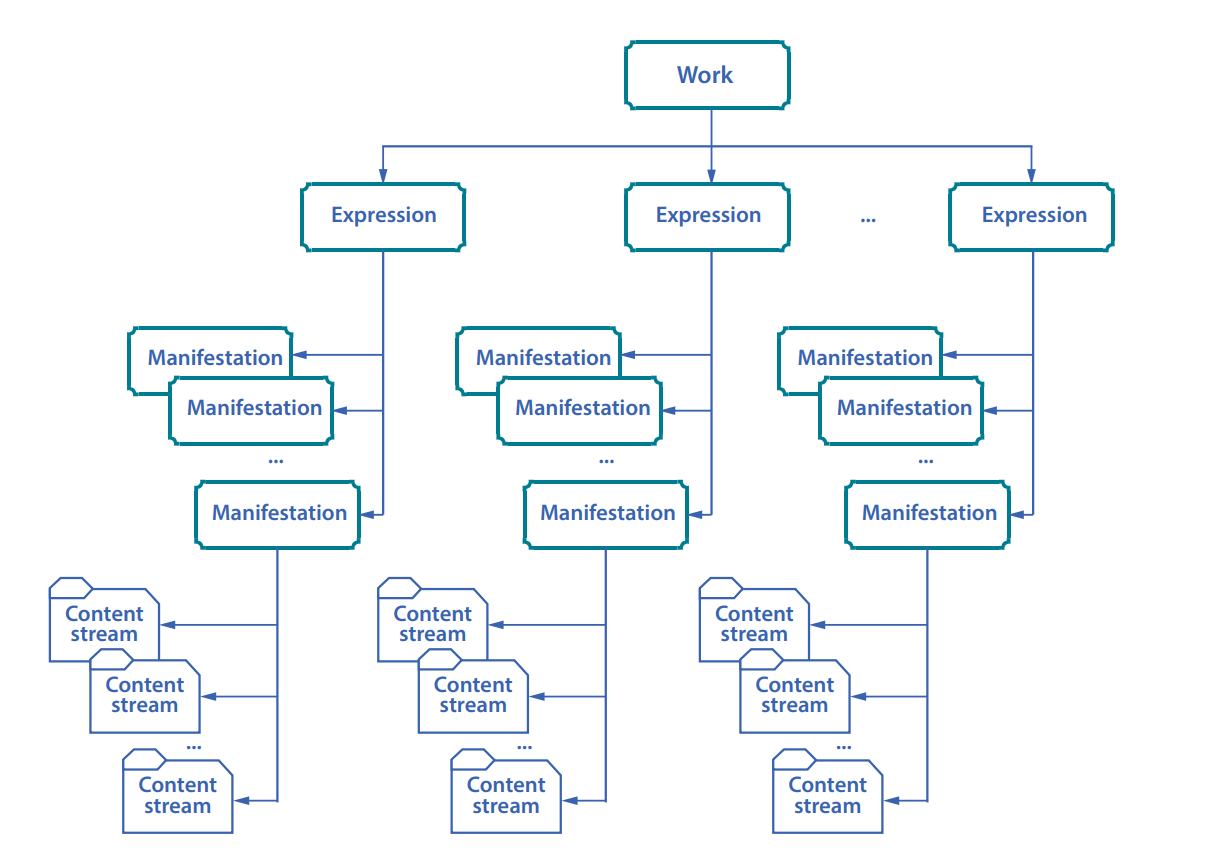
\includegraphics[width=0.625\linewidth]{gfx/content_modell.png}
        \caption{Work-Expressions-Manifestations-Content Stream Hierarchie}
        \label{fig:eu_wemi}
    \end{figure}
    
    \noindent
    Neben dem abstrakten Rahmen bestimmen \acs{FRBR} auch konkret die Abbildung der verfügbaren Metadaten der in Cellar geführten \textit{Werke}.
    Cellar präsentiert für die Darstellung der Metadaten folglich das Konzept eines ,,Notice``, welcher in unterschiedlichen Ausführungen, unterschiedlich granular die Metadaten zu einem \textit{Werk} abbildet.
    Dieses \textit{Notices} stellen dabei eine einheitliche Quelle dar, welche alle Metadaten des \textit{Werkes} und je nach Granularität, Metadaten von allen oder ausgewählten \textit{Expressionen} und \textit{Manifestationen} bündelt und nach dieser Hierarchie strukturiert bereitstellt.
    \cite[S. 31f]{eu_cellar}

\subsubsection{Cellar Formex}

    Das \acf{OP} startete bereits in dem Jahre 1985 mit der Produktion von \ac{SGML} Instanzen von -- im \ac{OJ} veröffentlichten -- Dokumenten, um den Austausch mit Auftragnehmern des \ac{OP} zu vereinfachen. \cite[75]{eu_cellar, eu_fmx4_intro}
    Diese verwendete Spezifikation hierfür wurde Formex (Formalised exchange of electronic documents) genannt.
    Nach der Veröffentlichung der Celex Version 3 (ab 04/1999) und unter dem nachlassenden Erfolg des \ac{SGML} Formates migrierte das Celex Format zu der kommenden Version 4 (ab 2004) zu dem strikterem \ac{XML} Dateiformat.
    Dies ermöglichte weiter auch die Adoption anderer entwickelter Standards und Werkzeugen, wie bspw. \ac{XSL}, \ac{XSLT} oder \ac{XSLFO} zur Darstellung und der weiteren Transformation der Daten für deren Anwendungs- oder Präsentationszwecke.
    Die endgültige Definition des Standards in der Version 4 setzt sich also aus den bestehenden Standards \ac{XML} und Unicode\footnote{zuvor ISO-2022} zusammen, auf Basis dessen eine Grammatik mittels \ac{XML}-Schema (ehemals \ac{DTD}) definiert wird. \cite{eu_fmx4_intro}
    
    \medskip
    Inhaltlich definiert Formex den logischen Aufbau, die Struktur aber auch den Inhalt  dieser \textit{Expressionen} der Rechtsakten.
    Das \ac{XML}-Schema bildet dabei alle strukturellen Aspekte wie Artikel, Absätze, Anhänge, etc. durch ein jeweiliges, in dem Schema definierten, Element ab. 
    Inhalte werden, integer zur \textit{Expression}, inklusive aller wichtigen Hinweise zur Textformatierung, Verweisen und Zitaten abgebildet. 
    Unter den Inhalten können -- entsprechend dieser Arbeit -- auch Anforderungen identifiziert werden, welche entweder, implizit in dem Gesetzestext (etwa einem Absatz) oder explizit durch eine aufgeführte Anforderung mit Anforderungsnummer\footnote{vgl. Anhänge von \acs{DVO} (\acs{EU}) 2017/373} in dem \textit{Manifestation} realisiert werden.

    \medskip
    Das Format ermöglicht es zumeist, einzelne strukturelle Komponenten und Elemente einer \textit{Manifestation} in Bezug auf das nächst übergeordnete Element zu referenzieren; eine absolute Referenzierung einzelner Elemente ist, über dessen Referenzierung der Position im Dokument\footnote{etwa mittels XPath}, nur in Ausnahmefällen möglich.
    Artikel und Absätze (\textsf{ARTICLE} und \textsf{PARAG} nach Formex) verfügen so über ein verpflichtendes geteiltes Attribut ,,\textsf{@IDENTIFIER}``, welches Auskunft über die Laufnummer in Bezug auf das aktuelle Dokument\footnote{\textit{Manifestation} umfasst mehrere Dokumente, bspw. Anhänge} bietet. 
    Explizite Anforderungen, welche in Anhängen dieses Dokumentes definiert sind, oder eine kleinere Granularität benötigen, lassen sich nur durch diese Information nicht identifizieren.
    Es gilt im Kommenden abzuwiegen, ob eine solche 

    \medskip
    Weiter werden auch Textabschnitte, welche nicht der Expression des \textit{Ursprungswerkes} entstammen, sondern der Expression eines Änderungstextes, in den entsprechenden \textit{Manifestationen} der \textit{Expressionen} der konsolidierten \textit{Werke} maschinenlesbar, aber der \textit{Expression} gegenüber integer, annotiert. 
    Im technischen Sinne bezeichnet dies sogenannte \ac{XML}-Processing Instructions, welche per se nicht einen Teil des \ac{XML} Inhaltes darstellen, aber weitere Verarbeitungsinformationen für Interpretation dieses bereitstellen. 
    Die entsprechenden Anweisungen ,,\textsf{CLG.MDFO}`` (Open) und ,,\textsf{CLG.MDFC}`` (Close) markieren dabei den jeweiligen Anfang und das Ende einer Änderung. 
    Attribute der Markierungen verweisen hierbei auf die jeweils andere Begrenzung, um eine Verwirrung bei mehreren oder verschachtelten Änderungen zu vermeiden.
    Zusätzlich hierzu verfügt die öffnende Anweisung über Informationen wie der Aktion der Änderung, ob es eine strukturelle oder inhaltliche Änderung ist und aus welchem \textit{Änderungswerk} diese Änderung hervorgeht. 
    \cite[vgl. S. 76 -- 79]{eu_fmx4_proc}
    
\section{Bewertung der Datenquelle}

    Das \acf{OP} bereitet Nutzer:innen durch Cellar und dessen untergeordnete Plattformen einen weitreichend und sehr tiefgehenden Zugang zu allen verfügbaren Informationen.
    % Dies stellt sehr wohl eine gesicherte Basis für beliebige Integrationen 
    Im Folgenden soll erörtert werden, inwiefern -- und mit welchem Aufwand -- diese Daten genutzt werden können, um die Automatisierung einer Impact-Analyse zu ATM/ANS-Equipment gemäß den in Kapitel \ref{model_anforderungen} dieser Arbeit definierten Anforderungen zu realisieren.
    
    Die Anforderungen, auf welchen die Analyse basiert, gehen zumeist aus der Verordnung \ac{DVO} (\ac{EU}) 2017/373 -- und künftig auch \ac{VO} (\ac{EU}) 2023/1769ff. -- hervor. 
    Auf dieser Basis stellt die \ac{EU}, und damit das \ac{OP}, die naheliegendste Quelle der Informationen dar, um eine möglichst hohe Integrität der Inhalte zu garantieren.
    Cellar verfügt weiter über alle relevanten Dokumente der Gesetzgebungsorgane, welche für die Erfüllung der Compliance relevant sein könnten. 

\pagebreak
\subsection{Integration in das erarbeitete Datenmodell}
    
    In Bezug auf die definierten Anforderungen bedarf es für eine ausreichende Abbildung der regulativen Anforderungen einer Eindeutigen Kennung, einer regulativen Quelle, einem nachvollziehbaren Lifecycle der einzelnen Verordnung sowie dessen Gültigkeitszeitraum.
    
\subsubsection{Eindeutige Kennung}
    
    Neben der eindeutigen Kennung der Anforderungsdokumente, bei welcher Cellar gleich mehrere eindeutige Identifikationsmöglichkeiten bietet, besteht unter Cellar keine Möglichkeit der eindeutigen Kennung einzelner Anforderungen, sowie diese nicht inhaltlich gegeben ist. 
    Die große Diversität der Anforderungsdokumente, welche alle u.U. eine Relevanz für die Nachweisführung mit sich tragen, bedürfen hier sehr ausgearbeitete Prozesse zur Erkennung und Referenzierung von neuen Anforderungen.  

\subsubsection{Regulative Quelle}
    
    Die regulative Quelle eines Textes, sowie vom ursprünglichem \textit{Werk} abweichend, lässt sich unter Cellar anhand von Metadaten oder Änderungsanweisungen im Inhalt ablesen.
    Im Falle der Metadaten beschreibt die Annotation die nächste übergeordnete Position der Änderung.
    Alternativ beschreiben inhaltlich Verarbeitungsanweisungen den betroffenen Bereich einer Änderung. 
    Sogleich eine Anforderung inhaltlich im Bereich einer, oder mehrerer, Änderungen liegt, gilt diese als von dieser betroffen.
    Dies erlaubt es sehr detailliert nachzuverfolgen, welche Texte, welche Änderungen an der Anforderungen bewirkt haben.
    In Bezug auf die Regulative Quelle im Sinne der Analyse gilt es lediglich die Differenz aller Änderungen in Bezug einer Anforderung zu bestimmen.
    Die Quelle der aktuellsten Änderung kann im Folgenden als regulative Quelle angenommen werden.

    \medskip
    Das Erheben der regulativ Quelle bedarf hier eines tiefen Verständnisses über die Struktur der \textit{Expression}, um sicherzustellen, dass Änderungsinformationen richtig auf modellierte Anforderungen abgebildet werden können.
    Sowie die Granularität der Anforderungsmodellierung nicht mit der Granularität der Änderungsmeldungen übereinstimmt, bedarf es der Translationsebene in Form einer (zweiten) inhaltlichen Impact-Analyse, welche in der Lage ist, Änderungen entsprechend auf die jeweiligen Anforderungen abzubilden.
    

\subsubsection{Inkrafttreten / Anwendungszeitraum}

    Analog zur Erhebung der Regulativen Quelle bedarf die Ermittlung des Anwendungszeitraums einer regulativen Anforderung, dessen genaue Historie aller Änderungen.
    Cellar stellt, wie oben beschrieben, im Rahmen der Metadaten-Änderungsannotationen Informationen über das Inkrafttreten der beschriebenen Änderungen zur Verfügung.
    Sowie die Implementierung es erlaubt, Änderungen den betroffenen Anforderungen zuzuweisen, kann auch dessen explizites Inkrafttreten der Anforderung zugewiesen werden.
    Dies weißt im Vergleich zum implizierten Annehmen des Anwendungszeitraums des Gesamtdokuments den Vorteil auf, dass Gesamtänderungen, welche sich heterogen auf die einzelnen Anforderungen auswirken, integrer abgebildet werden können.
    
\subsubsection{Lifecycle}

    Der Lifecycle einer Cellar Ressource kann allein an dessen Metadaten bestimmt werden.
    Neben teils weitreichenden Informationen über den Entwicklungsprozess der Anforderungsdokumenten\footnote{In Fällen von Rechtsakten, die durch das ordentliche Gesetzgebungsverfahren entwickelt wurden, umfasst Cellar zusätzliche Verfahrensinformationen. \cite[vgl.][]{2004R0552}}, bildet Cellars RDF-Graph alle wichtigen Ereignisse in Bezug auf das untersuchte Dokument ab.  
    Lediglich im Falle des Übertrags von bestehenden Anforderungen in ein neues Anforderungsdokument bedürfte es einer manuellen Migration.

    \vspace{3.5cm}
    \begin{figure}[hb]
        \centering
        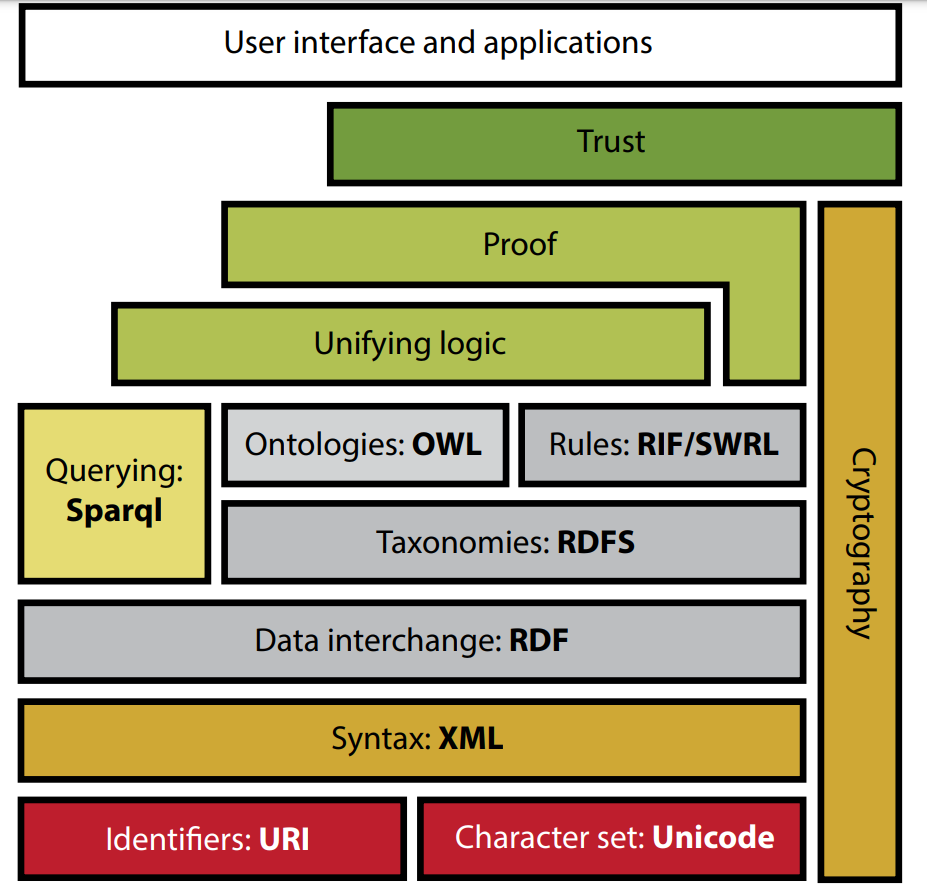
\includegraphics[width=.75\linewidth]{gfx/semantic_web_cake.png}
        \caption{Semantic Web Tech-Stack}
        \cite[10]{eu_cellar} (Ursprung nicht mehr verfügbar)
        \label{fig:semantic}
    \end{figure}
    